%Corps du document :
%\setlength{\parindent}{1cm}    

\section{Cadre du projet}

Le but du projet ``Système d'Information Urbanisé et SOA'' est de mettre en application la démarche et
les méthodes de conception de systèmes d'information vues en cours dans le cadre d'une architecture répartie.

\subsection{Thème du projet}

Il s'agira de fournir une solution logicielle pour ``la gestion des contacts commerciaux'' d'une banque,
en apportant une aide à ses agents commerciaux pour :

\begin{itemize}
\item Identifier et définir les contacts qu'ils doivent avoir avec leurs clients,
\item Permettre au chef d'agence de répartir ces contacts entre ses collaborateurs,
\item Prendre les rendez-vous et tenir leurs agendas,
\item Préparer ces rendez-vous et les projets de proposition en fonction des clients,
\item Construire les entretiens lors des rendez-vous et déclarer les résultats obtenus,
\item Suivre la réalisation des contacts programmés.
\end{itemize}

\subsection{Phases du projet}

Ce projet se déroulera en 3 phases :

\begin{itemize}
\item La conception d'ensemble de l'architecture applicative,
\item La conception détaillée des applications,
\item La répartition des composants sur l'architecture n-tiers.
\end{itemize}

\subsection{Outils de suivi}

\begin{itemize}
\item Nous utiliserons l'outil de gestion de projet \textbf{RedMine} pour la conduite de projet, la répartition et l'organisation des tâches, et l'établissement d'un planning prévisionnel.
\item Notre RedMine sera interfacé avec l'outil de gestion de révision \textbf{Git} et son webservice \textbf{GitHub.com} pour le suivi de l'évolution des documents et son environnement de travail collaboratif distribué.
\end{itemize}

\section{Objectifs en termes de produits finis}

\subsection{Document d'Initialisation}

Le présent document vise à définir l'organisation et la répartition des tâches du projet avec une estimation initiale des charges pour dimensionner le projet et démarrer les activités.

\subsection{Compte-Rendu du projet}

Le Compte-Rendu du projet est composé de :

\begin{itemize}
\item \textbf{Conception d'ensemble} : Elle permet d'identifier les évolutions de l'architecture applicative, nécessaires pour satisfaire les besoins des utilisateurs. Elle comportera :

\begin{itemize}
\item Les modèles conceptuels de données du domaine étudié,
\item Le découpage des cas d'utilisation représentatifs en sénarios élémentaires, à l'aide de diagrammes d'activité et diagrammes de séquence système,
\item La définition générale des blocs du noyau applicatif à l'aide de modèles de données découpés en blocs,
\item L'identification des cycles de vie complexe des objets métiers à l'aide d'un diagramme d'état d'objet métier (pour l'objet Contact),
\item La dynamique de l'architecture, à savoir l'identification des principaux flux d'information échangés entre les utilisateurs et les blocs de l'architecture logique (diagrammes de séquence) et des principaux flux multi blocs, avec synthèse et validation de l'architecture de services (diagramme de collaboration),
\item Le choix de l'environnement technique retenu.
\end{itemize}

\item \textbf{Conception détaillée} : Elle permet d'identifier et de spécifier les composants nécessaires pour automatiser tout ou partie des outils à utiliser dans le cadre des cas d'utilisation identifiés. Elle comportera :

\begin{itemize}
\item Les composants de l'IHM, avec liste des dialogues/EdF, la description des fenêtres de dialogue et la liste des services invoqués,
\item Les composants du noyaux applicatif, avec la spécification des services métiers et des services objets métiers.
\end{itemize}

\item \textbf{Architecture de l'application} : La répartition des composants du noyau applicatif sur une architecture n-tiers.
\end{itemize}

\subsection{Présentation finale}

Une copie des supports de présentation sera fournie.

\subsection{Bilan du projet}

Une synthèse retrospective sur le déroulement du projet.

\section{Organisation des tâches}

\subsection{Répartition des tâches}

\begin{itemize}
\item Conception d'ensemble du système

\begin{itemize}
\item Analyse des modèles conceptuels proposés (assigné à \textbf{Xavier Sauvagnat})
\item Etablissement des diagrammes d'activités (assigné à \textbf{Matthieu Coquet})
\item Etablissement des diagrammes de séquences systèmes (assigné à \textbf{Alexandre Lefoulon})
\item Identifier et définir les blocs applicatifs

\begin{itemize}
\item Etablissement du modèle de données découpés en blocs (assigné à \textbf{Alexandre Lefoulon})
\end{itemize}

\item Identifier les cycles de vie des objets métiers

\begin{itemize}
\item Etablissement du diagramme d'état d'objet métier pour l'objet Contact (assigné à \textbf{Jan Keromnes})
\end{itemize}

\item Détermination des flux de l'architecture

\begin{itemize}
\item Etablissement d'un diagramme de séquence (assigné à \textbf{Quentin Calvez})
\item Etablissement d'un diagramme de collaboration(assigné à \textbf{Thaddee Tyl})
\end{itemize}

\item Choix de l'environnement technique (assigné à \textbf{Matthieu Coquet})

\end{itemize}
\item Conception détaillée

\begin{itemize}
\item Interface utilisateur

\begin{itemize}
\item Diagrammes EdF (assigné à \textbf{Jan Keromnes})
\item Description des fenêtres (assigné à \textbf{Quentin Calvez})
\item Services IHM (assigné à \textbf{Jan Keromnes})
\end{itemize}

\item Couche noyau

\begin{itemize}
\item Spécification des SM (assigné à \textbf{Xavier Sauvagnat})
\item Spécification des SOM (assigné à \textbf{Alexandre Lefoulon})
\end{itemize}

\end{itemize}

\item Architecture technique et répartition du SI

\begin{itemize}
\item Choix architecture Centralisée/Réparties (assigné à \textbf{Quentin Calvez})
\item Choix de la répartition des composants applicatifs (assigné à \textbf{Thaddee Tyl})
\item Détermination des principaux flux au sein de l'application, CRUD (assigné à \textbf{Jan Keromnes})
\end{itemize}

\end{itemize}

\subsection{Evaluation des charges}

\begin{itemize}
\item Conception d'ensemble du système

\begin{itemize}
\item Analyse des modèles conceptuels proposés (temps estimé \textbf{3h00})
\item Etablissement des diagrammes d'activités (temps estimé \textbf{4h00})
\item Etablissement des diagrammes de séquences systèmes (temps estimé \textbf{3h00})

\item Identifier et définir les blocs applicatifs

\begin{itemize}
\item Etablissement du modèle de données découpés en blocs (temps estimé \textbf{3h00})
\end{itemize}

\item Identifier les cycles de vie des objets métiers

\begin{itemize}
\item Etablissement du diagramme d'état d'objet métier pour l'objet Contact (temps estimé \textbf{2h00})
\end{itemize}

\item Détermination des flux de l'architecture

\begin{itemize}
\item Etablissement d'un diagramme de séquence (temps estimé \textbf{3h00})
\item Etablissement d'un diagramme de collaboration(temps estimé \textbf{3h00})
\end{itemize}

\item Choix de l'environnement technique (temps estimé \textbf{3h00})

\end{itemize}

\item Conception détaillée

\begin{itemize}
\item Interface utilisateur

\begin{itemize}
\item Diagrammes EdF (temps estimé \textbf{5h00})
\item Description des fenêtres (temps estimé \textbf{5h00})
\item Services IHM (temps estimé \textbf{2h00})
\end{itemize}

\item Couche noyau

\begin{itemize}
\item Spécification des SM (temps estimé \textbf{4h00})
\item Spécification des SOM (temps estimé \textbf{4h00})
\end{itemize}

\end{itemize}

\item Architecture technique et répartition du SI

\begin{itemize}
\item Choix architecture Centralisée/Réparties (temps estimé \textbf{4h00})
\item Choix de la répartition des composants applicatifs (temps estimé \textbf{4h00})
\item Détermination des principaux flux au sein de l'application, CRUD (temps estimé \textbf{4h00})
\end{itemize}

\end{itemize}

\paragraph{Estimation totale} La charge totale estimée pour ce projet est de \textbf{66 heure/hommes}, calculé avec des marges opérationnelles de 15\%.

\section{Diagramme de Gantt}

\begin {center}
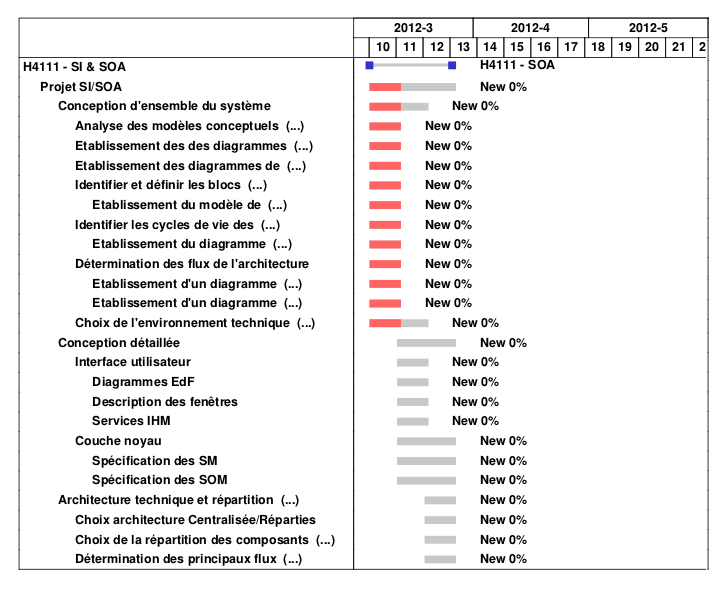
\includegraphics[width=\textwidth]{gantt.png}
\end {center}
